% Options for packages loaded elsewhere
\PassOptionsToPackage{unicode}{hyperref}
\PassOptionsToPackage{hyphens}{url}
\PassOptionsToPackage{dvipsnames,svgnames,x11names}{xcolor}
%
\documentclass[
  letterpaper,
  DIV=11,
  numbers=noendperiod]{scrartcl}

\usepackage{amsmath,amssymb}
\usepackage{setspace}
\usepackage{iftex}
\ifPDFTeX
  \usepackage[T1]{fontenc}
  \usepackage[utf8]{inputenc}
  \usepackage{textcomp} % provide euro and other symbols
\else % if luatex or xetex
  \usepackage{unicode-math}
  \defaultfontfeatures{Scale=MatchLowercase}
  \defaultfontfeatures[\rmfamily]{Ligatures=TeX,Scale=1}
\fi
\usepackage{lmodern}
\ifPDFTeX\else  
    % xetex/luatex font selection
\fi
% Use upquote if available, for straight quotes in verbatim environments
\IfFileExists{upquote.sty}{\usepackage{upquote}}{}
\IfFileExists{microtype.sty}{% use microtype if available
  \usepackage[]{microtype}
  \UseMicrotypeSet[protrusion]{basicmath} % disable protrusion for tt fonts
}{}
\makeatletter
\@ifundefined{KOMAClassName}{% if non-KOMA class
  \IfFileExists{parskip.sty}{%
    \usepackage{parskip}
  }{% else
    \setlength{\parindent}{0pt}
    \setlength{\parskip}{6pt plus 2pt minus 1pt}}
}{% if KOMA class
  \KOMAoptions{parskip=half}}
\makeatother
\usepackage{xcolor}
\setlength{\emergencystretch}{3em} % prevent overfull lines
\setcounter{secnumdepth}{-\maxdimen} % remove section numbering
% Make \paragraph and \subparagraph free-standing
\makeatletter
\ifx\paragraph\undefined\else
  \let\oldparagraph\paragraph
  \renewcommand{\paragraph}{
    \@ifstar
      \xxxParagraphStar
      \xxxParagraphNoStar
  }
  \newcommand{\xxxParagraphStar}[1]{\oldparagraph*{#1}\mbox{}}
  \newcommand{\xxxParagraphNoStar}[1]{\oldparagraph{#1}\mbox{}}
\fi
\ifx\subparagraph\undefined\else
  \let\oldsubparagraph\subparagraph
  \renewcommand{\subparagraph}{
    \@ifstar
      \xxxSubParagraphStar
      \xxxSubParagraphNoStar
  }
  \newcommand{\xxxSubParagraphStar}[1]{\oldsubparagraph*{#1}\mbox{}}
  \newcommand{\xxxSubParagraphNoStar}[1]{\oldsubparagraph{#1}\mbox{}}
\fi
\makeatother


\providecommand{\tightlist}{%
  \setlength{\itemsep}{0pt}\setlength{\parskip}{0pt}}\usepackage{longtable,booktabs,array}
\usepackage{calc} % for calculating minipage widths
% Correct order of tables after \paragraph or \subparagraph
\usepackage{etoolbox}
\makeatletter
\patchcmd\longtable{\par}{\if@noskipsec\mbox{}\fi\par}{}{}
\makeatother
% Allow footnotes in longtable head/foot
\IfFileExists{footnotehyper.sty}{\usepackage{footnotehyper}}{\usepackage{footnote}}
\makesavenoteenv{longtable}
\usepackage{graphicx}
\makeatletter
\def\maxwidth{\ifdim\Gin@nat@width>\linewidth\linewidth\else\Gin@nat@width\fi}
\def\maxheight{\ifdim\Gin@nat@height>\textheight\textheight\else\Gin@nat@height\fi}
\makeatother
% Scale images if necessary, so that they will not overflow the page
% margins by default, and it is still possible to overwrite the defaults
% using explicit options in \includegraphics[width, height, ...]{}
\setkeys{Gin}{width=\maxwidth,height=\maxheight,keepaspectratio}
% Set default figure placement to htbp
\makeatletter
\def\fps@figure{htbp}
\makeatother
% definitions for citeproc citations
\NewDocumentCommand\citeproctext{}{}
\NewDocumentCommand\citeproc{mm}{%
  \begingroup\def\citeproctext{#2}\cite{#1}\endgroup}
\makeatletter
 % allow citations to break across lines
 \let\@cite@ofmt\@firstofone
 % avoid brackets around text for \cite:
 \def\@biblabel#1{}
 \def\@cite#1#2{{#1\if@tempswa , #2\fi}}
\makeatother
\newlength{\cslhangindent}
\setlength{\cslhangindent}{1.5em}
\newlength{\csllabelwidth}
\setlength{\csllabelwidth}{3em}
\newenvironment{CSLReferences}[2] % #1 hanging-indent, #2 entry-spacing
 {\begin{list}{}{%
  \setlength{\itemindent}{0pt}
  \setlength{\leftmargin}{0pt}
  \setlength{\parsep}{0pt}
  % turn on hanging indent if param 1 is 1
  \ifodd #1
   \setlength{\leftmargin}{\cslhangindent}
   \setlength{\itemindent}{-1\cslhangindent}
  \fi
  % set entry spacing
  \setlength{\itemsep}{#2\baselineskip}}}
 {\end{list}}
\usepackage{calc}
\newcommand{\CSLBlock}[1]{\hfill\break\parbox[t]{\linewidth}{\strut\ignorespaces#1\strut}}
\newcommand{\CSLLeftMargin}[1]{\parbox[t]{\csllabelwidth}{\strut#1\strut}}
\newcommand{\CSLRightInline}[1]{\parbox[t]{\linewidth - \csllabelwidth}{\strut#1\strut}}
\newcommand{\CSLIndent}[1]{\hspace{\cslhangindent}#1}

\KOMAoption{captions}{tableheading}
\makeatletter
\@ifpackageloaded{caption}{}{\usepackage{caption}}
\AtBeginDocument{%
\ifdefined\contentsname
  \renewcommand*\contentsname{Table of contents}
\else
  \newcommand\contentsname{Table of contents}
\fi
\ifdefined\listfigurename
  \renewcommand*\listfigurename{List of Figures}
\else
  \newcommand\listfigurename{List of Figures}
\fi
\ifdefined\listtablename
  \renewcommand*\listtablename{List of Tables}
\else
  \newcommand\listtablename{List of Tables}
\fi
\ifdefined\figurename
  \renewcommand*\figurename{Figure}
\else
  \newcommand\figurename{Figure}
\fi
\ifdefined\tablename
  \renewcommand*\tablename{Table}
\else
  \newcommand\tablename{Table}
\fi
}
\@ifpackageloaded{float}{}{\usepackage{float}}
\floatstyle{ruled}
\@ifundefined{c@chapter}{\newfloat{codelisting}{h}{lop}}{\newfloat{codelisting}{h}{lop}[chapter]}
\floatname{codelisting}{Listing}
\newcommand*\listoflistings{\listof{codelisting}{List of Listings}}
\makeatother
\makeatletter
\makeatother
\makeatletter
\@ifpackageloaded{caption}{}{\usepackage{caption}}
\@ifpackageloaded{subcaption}{}{\usepackage{subcaption}}
\makeatother

\ifLuaTeX
  \usepackage{selnolig}  % disable illegal ligatures
\fi
\usepackage{bookmark}

\IfFileExists{xurl.sty}{\usepackage{xurl}}{} % add URL line breaks if available
\urlstyle{same} % disable monospaced font for URLs
\hypersetup{
  pdftitle={Chapter0},
  colorlinks=true,
  linkcolor={blue},
  filecolor={Maroon},
  citecolor={blue},
  urlcolor={Blue},
  pdfcreator={LaTeX via pandoc}}


\title{Chapter0}
\author{}
\date{}

\begin{document}
\maketitle

\renewcommand*\contentsname{Table of contents}
{
\hypersetup{linkcolor=}
\setcounter{tocdepth}{3}
\tableofcontents
}

\setstretch{2}
\section{1 Motivation}\label{motivation}

Footwear examination is important to forensic investigation. The
features provided by footwear prints are known as class characteristics:
they may be shared by many shoes of the same make and model, but are
useful for narrowing down a subject pool and providing some association
between a suspect and the
scene\textsuperscript{\citeproc{ref-bodziak2017footwear}{1}}. Collection
and processing of footwear data require large amounts of human labor,
hence, automating the the process of identification class
characteristics is essential. With advances in neural network-based
vision models, automated process has become feasible.

\section{2 Neural Network Vision
Models}\label{neural-network-vision-models}

Modern neural network-based vision models are mainly built on two
categories of architectures: convolutional neural networks and
attention-based networks. Although they use different mechanisms, these
architectures are used as backbones to extract features from images.
These features can be used by downstream task-specific modules, which
are also referred to as heads. Task-specific heads are selected
depending on the objective of the model. For example, in an image
classification task, a classification head is attached to the backbone
to predict image-level categories. In an object detection task,
detection heads are used to predict both object classes and bounding box
locations. A diagram of a neural network is shown in
Figure~\ref{fig-1-vision-model-diagram}.

\begin{figure}

\centering{

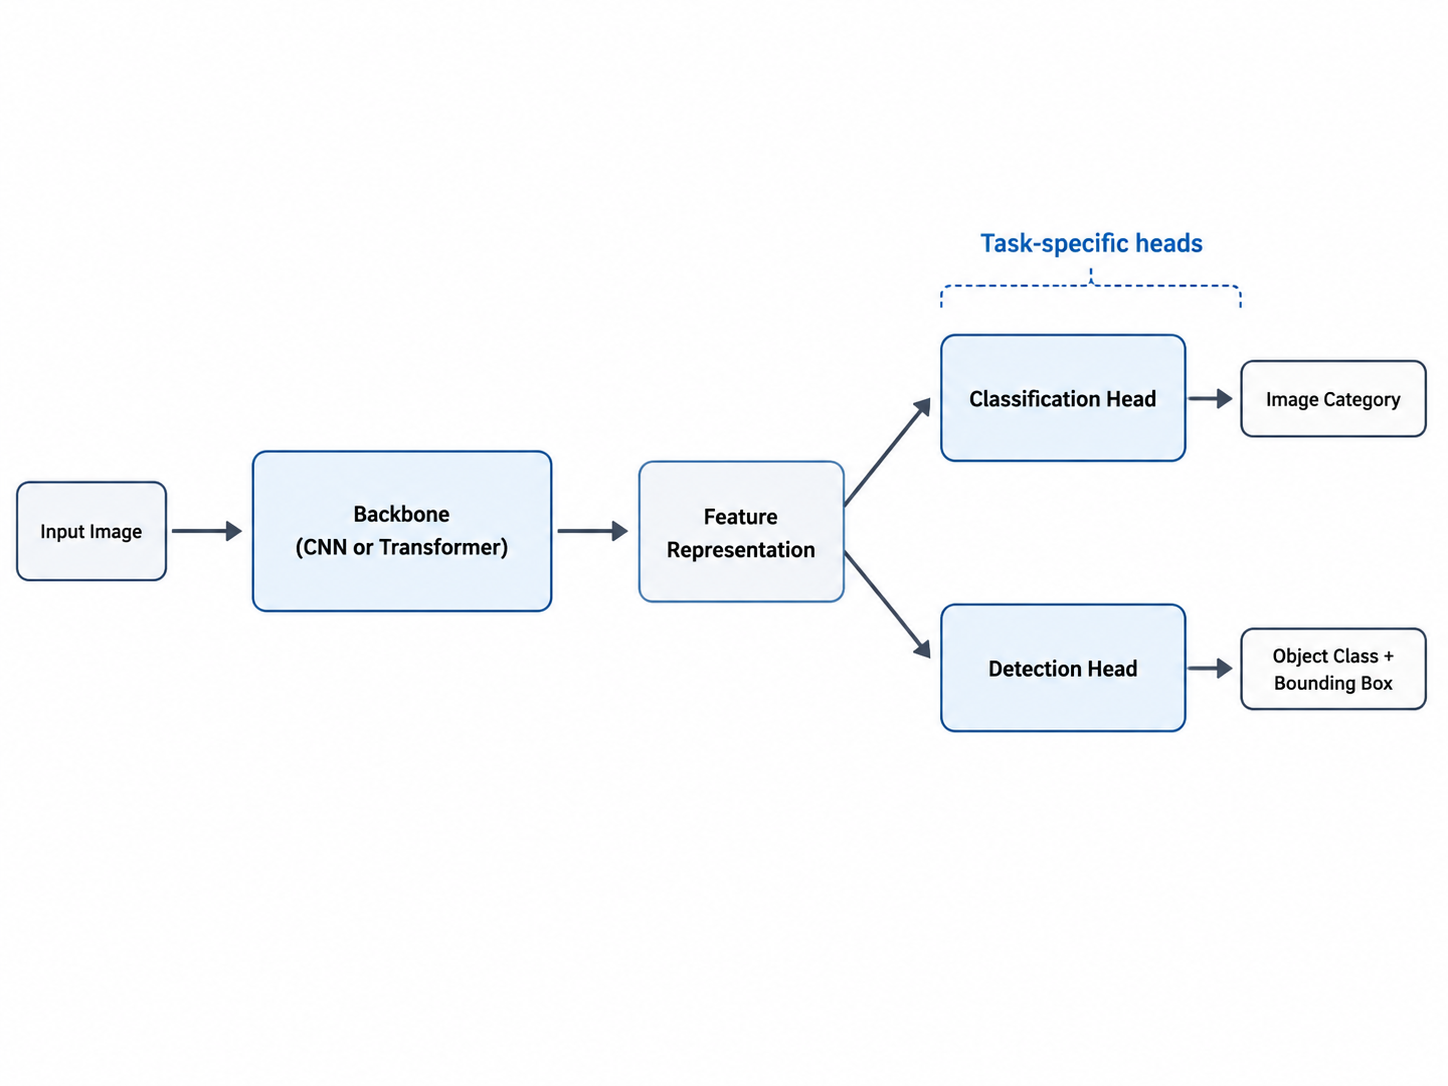
\includegraphics[width=4.16667in,height=\textheight]{chapter0_img/nn-diagram.png}

}

\caption{\label{fig-1-vision-model-diagram}Vision model diagram}

\end{figure}%

\subsection{2.1 Convolutional-based Vision
Models}\label{convolutional-based-vision-models}

Convolutional neural networks (CNNs) are one of the most widely used
neural network architectures. The development of convolutional neural
networks can be traced to biologically inspired models of vision.

A hierarchy model\textsuperscript{\citeproc{ref-Hubel1962}{2}}
\textsuperscript{\citeproc{ref-Hubel1965}{3}} proposed that the neural
network in the visual cortex are structured in a hierarchical way:
responses from low level cells are integrated by higher-level cells, so
that more complex visual features of larger receptive field can be
detected with great tolerance to positional shifts. Based on this idea,
Fukushima proposed the
Neocognitron\textsuperscript{\citeproc{ref-fukushima1980neocognitron}{4}},
an early neural network model for visual pattern recognition.
Figure~\ref{fig-neocognitron} shows how the Neocognitron structure
corresponding to the biological hierarchy visual model. In the
Neocognitron, the (\(U_s\)) and (\(U_c\)) layers provide an artificial
analogy to simple and complex cells. S-cell layers detect local visual
feature, while C-cell layers combine nearby responses. A complex visual
representation is built by repeating the S-cell followed by C-cell
strucuter.

\begin{figure}

\centering{

\includegraphics{chapter0_img/neocognition.png}

}

\caption{\label{fig-neocognitron}Correspondence between the hierarchy
model by Hubel and Wiesel, and the neural network of the neocognitron}

\end{figure}%

While the Neocognitron is considered as a biologically inspired
precursor, LeNet, proposed by LeCun, represented a early form of modern
convolutional neural networks. LeNet established a basic structure for
later CNN architectures and enabled image features to be learned
directly from image data. In this structure, convolutional filters
(Figure~\ref{fig-2-convolution-operation}) are applied to local regions
of the input image to detect spatial patterns.

\begin{figure}

\centering{

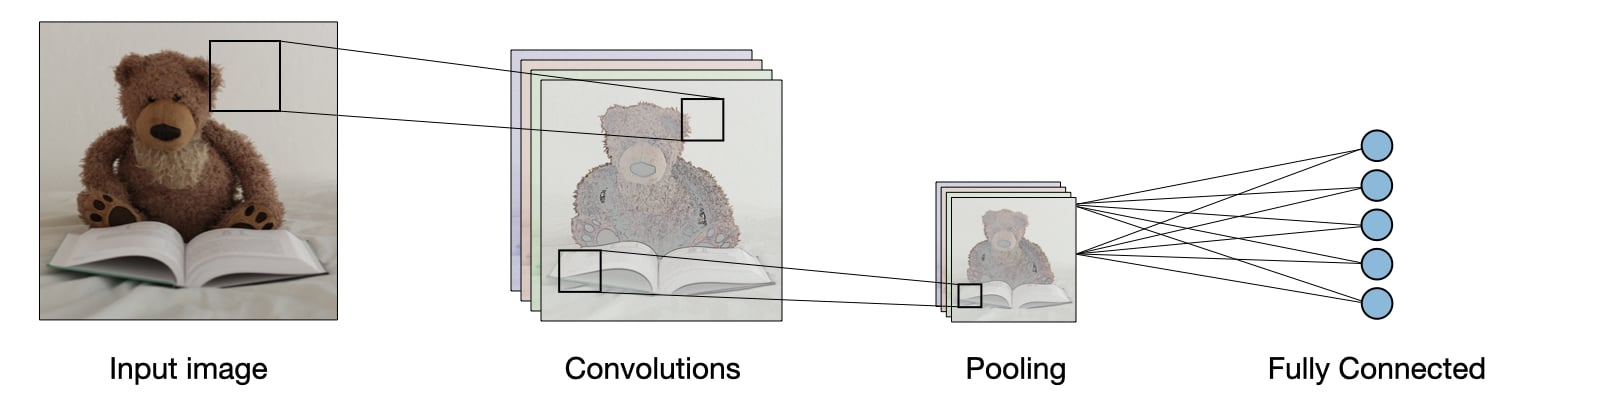
\includegraphics[width=4.16667in,height=\textheight]{chapter0_img/convolution-operation.jpeg}

}

\caption{\label{fig-2-convolution-operation}Convolution operation}

\end{figure}%

As a filter moves across the image, it computes responses to local
visual patterns and produces a feature map that represents the strength
of the filter response at different spatial locations. The filter plays
a role similar to S-cells in the Neocognitron, in that they respond to
local visual patterns and provide the basis for progressively more
complex feature representations.

The use of local convolutional filters and shared weights gives CNNs
strong image-specific inductive biases. Local convolutional filters
implies the assumption that nearby pixels are more likely to be related
than distant pixels. Shared weights allow the same filter to be reused
across spatial locations, this design supports translation equivariance,
in which a spatial shift in the input tends to produce a corresponding
shift in the feature response. By stacking multiple convolutional
layers, CNNs can gradually integrate local patterns into more complex
and abstract visual representations. This local-to-global organization
is conceptually related to hierarchical processing in the biological
visual system.

\subsection{2.2 Attention-based Vision
Models}\label{attention-based-vision-models}

Attention-based vision models are another major class of neural
network-based models. Attention mechanism is introduce in a natural
language processing model named
Transformer\textsuperscript{\citeproc{ref-transformer}{5}}. The
attention mechanism allows a model to assign different weights to
different parts of the input. Heavier weights indicate relevant parts
contributing more to the learned representation, which directly models
global context. This idea was later adapted to vision modeling through
the Vision Transformer\textsuperscript{\citeproc{ref-vit}{6}} (ViT). The
Vision Transformer inherits the attention mechanism to model region
relevance. An input image is represented as a sequence of segmented
visual patches, and the patches are assigned attention weights according
to their relevance to the representation. In this way, the model learns
relationships among different patches and captures long-range
dependencies across the image. This differs from CNNs, which primarily
learn local patterns through convolutional operations and gradually
build broader spatial context though stacking layers.

The diagram is shown in Figure~\ref{fig-vit}。 The input image is first
split into image patches. These patches are embedded as tokens and then
processed by the self-attention module. Self-attention assigns different
weights to different patches according to their relevance. The output
attention maps show the spatial distribution of these attention weights
across the image.

\begin{figure}

\centering{

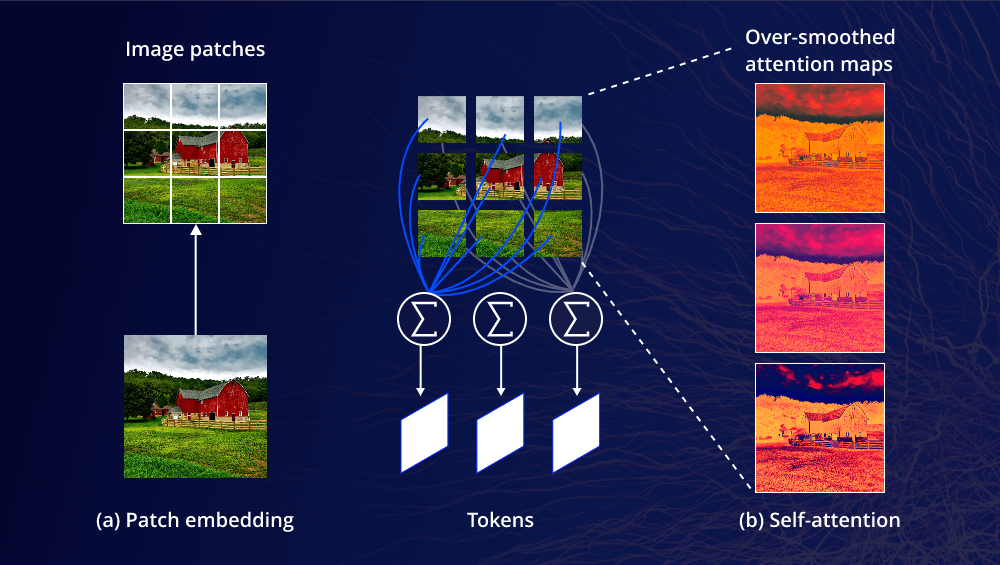
\includegraphics[width=4.16667in,height=\textheight]{chapter0_img/vision-transformer-model-2.png}

}

\caption{\label{fig-vit}Vision Transformer}

\end{figure}%

While CNNs assumes that local regions are more likely to be related by
employing local filters, the Vision Transformer does not impose
receptive fields and models global context with a direct mechanism.
Therefore, the Vision Transformer often requires large-scale training
data to learn robust visual representations.

\subsection{2.3 Heads and Transfer
Learning}\label{heads-and-transfer-learning}

Both CNN-based and attention-based architectures can be used to extract
image features. However, these features must be used by a task-specific
head to complete a particular task. For image classification, a
classification head maps the features to category predictions. For
object detection, detection heads use the feature representation to
predict both object categories and locations.

In a specific project, the task-specific head is usually selected or
modified according to the objective of the study. For example, in an
image classification task with seven categories, the final
classification head need to be replaced by a seven-class classifier. The
model is then trained by minimizing a task-specific loss function, such
as a classification loss for category prediction.

In many applied vision projects, the computing resource or the number of
project-specific training images are limited. Therefore, transfer
learning is a commonly used strategy in the training to improve
efficiency and performance. In transfer learning, a model is first
pretrained on a large scale dataset, such as
ImageNet\textsuperscript{\citeproc{ref-imagenet-transferlearning}{7}}
for image classification, and then adapted to the target dataset.
Through pretraining, the backbone learns general visual features, such
as edges, textures, and shapes, are considered transferable across
different image datasets and vision
tasks\textsuperscript{\citeproc{ref-transfer-learning}{8}}. Then the
task-specific head can be replaced or fine-tuned for the new task. The
task-specific model is further trained using the target data. During the
training, the pretrained backbones can be freezed or fine-tuned together
with the new head, because it was found that features in deeper layers
become increasingly specific to the original
task\textsuperscript{\citeproc{ref-transfer-learning}{8}}. The transfer
learning diagram is shown in Figure~\ref{fig-transfer-learning}.

\begin{figure}

\centering{

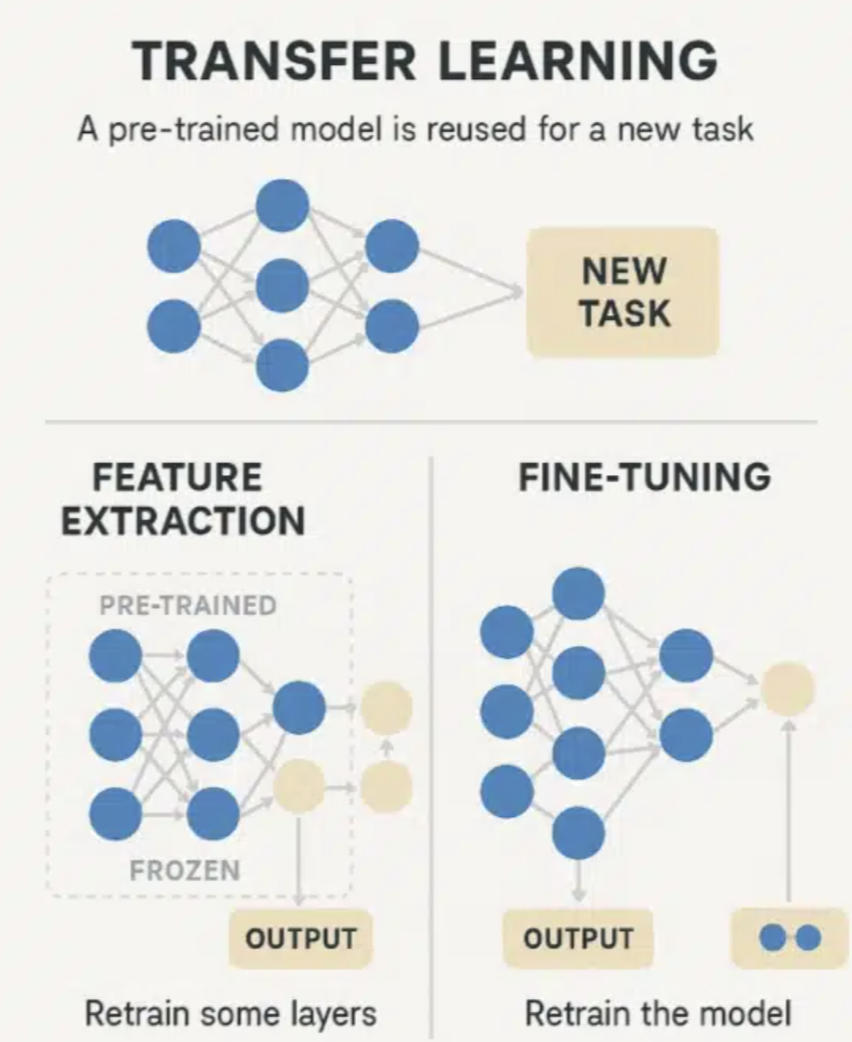
\includegraphics[width=\textwidth,height=2.08333in]{chapter0_img/transfer-learning.png}

}

\caption{\label{fig-transfer-learning}Transfer learning}

\end{figure}%

Previous studies have demonstrated that transfer learning is effective,
especially across visual network architectures and
tasks\textsuperscript{\citeproc{ref-vit}{6}}
\textsuperscript{\citeproc{ref-R-CNN}{9}}\textsuperscript{\citeproc{ref-vgg}{10}}
\textsuperscript{\citeproc{ref-resnet}{11}}.

The goal of the present study is to locate and classify footwear class
characteristics. These characteristics often consist of geometric
patterns that contain both local features and broader spatial context.
For example, recognizing a circular pattern requires the model to
identify local curvature as well as the overall closed shape. Therefore,
both CNN-based and attention-based models are considered suitable for
this task. Given the limited amount of labeled training data, transfer
learning is employed to improve model performance.

\section{3 Image Classification}\label{image-classification}

Image classification is a fundamental task in computer vision because it
provides a basic framework for learning and evaluating visual feature
representations. A classification dataset consists of images and their
corresponding class labels, which are assigned to the entire image. In a
classification model, a classification head uses these features that
output from a backbone to predict the image category. Many widely used
backbones were originally developed and evaluated on image
classification datasets. The representations learned through
classification later became the foundation for models used in various
vision tasks. This section reviews four representative architectures:
AlexNet\textsuperscript{\citeproc{ref-alexnet}{12}},
VGG\textsuperscript{\citeproc{ref-vgg}{10}},
ResNet\textsuperscript{\citeproc{ref-resnet}{11}}, and the Vision
Transformer\textsuperscript{\citeproc{ref-vit}{6}}. These architectures
illustrate important developments in convolutional and attention-based
visual modeling.

\subsection{3.1 Data}\label{data}

An image classification dataset consists of images and their labels. In
the simplest case of single label task, each image is assigned to one
category. The labeled images are divided into training, validation, and
test sets. The training set is used to optimize the model parameters by
minimizing a classification loss function, which measures the difference
between the predicted class and observed labels. The validation set is
used to identify potential overfitting, and the test set consists of
held out images which are reserved for the final evaluation. During
training, both the backbone and the classification head can be
optimized: the backbone learns visual feature representations, and the
classification head maps these representations to class predictions.

\subsection{3.2 Architectures}\label{architectures}

\subsubsection{3.2.1 AlexNet}\label{alexnet}

AlexNet, introduced by
Krizhevsky\textsuperscript{\citeproc{ref-alexnet}{12}}, was an
influential convolutional neural network. It demonstrated that a large
convolutional network could be successfully trained on a large-scale
image dataset, and hierarchical visual features could be learned
directly from image data.

The success helps to establish deep CNNs as a central approach in
computer vision. Its architecture incorporated several techniques that
facilitated large-scale CNN training to allow effective robust feature
representation learning and large scale image classification.

Although transfer learning had been studied earlier than AlexNet, the
success of AlexNet contributed to the prevalence of transfer learning.
Fine-tuning a deep neural network initialized with pretrained weights,
such as those from AlexNet, has been shown to outperform training the
same network from random
initialization\textsuperscript{\citeproc{ref-transfer-learning}{8}}.
Transfer learning with networks pretrained on large-scale datasets
therefore provides a general paradigm for various vision-related tasks.

Another practice popularized by AlexNet was data augmentation. Data
augmentation artificially enlarges the training dataset using
label-preserving transformations, which helps the network learn more
general features and reduces overfitting. AlexNet applied several
augmentation techniques (Figure~\ref{fig-augmentation}), including
random cropping, horizontal reflection, and RGB intensity perturbation.
These operations do not change the semantic content of the image but
expose the model to different variations of the same object, improving
its ability to generalize to unseen data.

\begin{figure}

\centering{

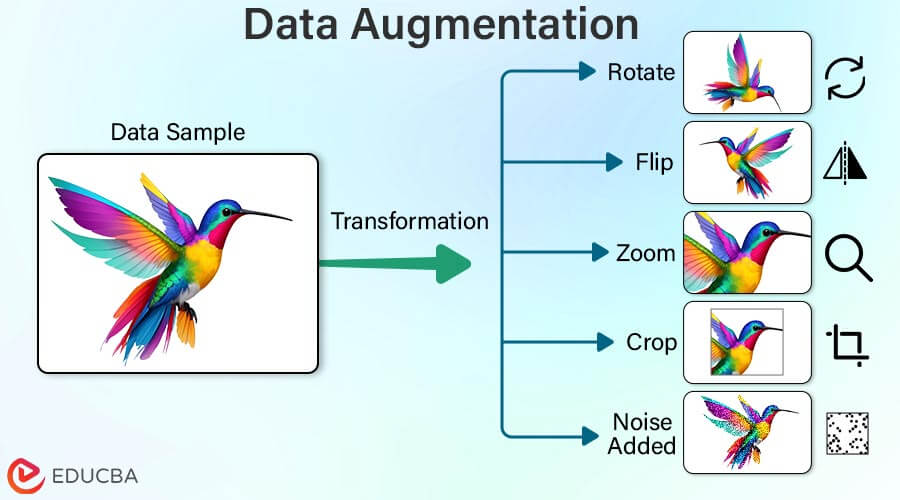
\includegraphics[width=\textwidth,height=2.08333in]{chapter0_img/augmentation.jpg}

}

\caption{\label{fig-augmentation}Data augmentation}

\end{figure}%

\subsubsection{3.2.2 VGG}\label{vgg}

Building on the success of AlexNet, deeper networks was proposed to
improve feature learning, representatives of the deep networks are the
configurations proposed by Simonyan et
al.\textsuperscript{\citeproc{ref-vgg}{10}}. These configurations became
widely know as VGG networks, named after the Visual Geometry Group at
the University of Oxford. The two commonly known architectures are
VGG-16 and VGG-19, which use a simple and uniform design based on
repeated small convolutional filters (3 by 3) and contain 16 and 19
learnable layers, respectively. Compared with AlexNet, which contains
eight learnable layers, VGG substantially increased network depth, see
Figure~\ref{fig-layer_diff}. The study demonstrated that this deeper
architecture improved image classification performance, suggesting an
improved ability to learn discriminative visual representations.

\begin{figure}

\centering{

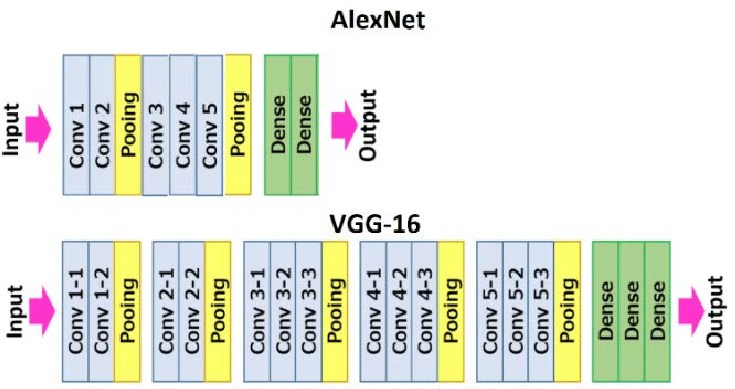
\includegraphics[width=\textwidth,height=2.08333in]{chapter0_img/layer_diff.png}

}

\caption{\label{fig-layer_diff}AlexNet: 8 learnable layers, VGG-16: 16
learnable layers}

\end{figure}%

\subsubsection{3.2.3 ResNet}\label{resnet}

The deep layer design of CNNs brought an unexpected degradation despite
better performance. It was found that adding more identical mapping
layers could result in higher training error as well as test
error\textsuperscript{\citeproc{ref-layerdiff}{13}}. This observation
suggests that the performance degradation is primarily associated with
optimization difficulties rather than overfitting.

ResNet architectures\textsuperscript{\citeproc{ref-resnet}{11}}
addressed the problem by introducing a deep residual learning module.
This module adds a shortcut connection to add the input directly to the
output of a few layers. The design makes optimization easier by learning
the residual modification relative to the input rather than the full
mapping. If the modification is small, as in an identity mapping, the
optimization becomes much easier than in the normal design
(Figure~\ref{fig-residual}).

ResNet networks has five standard variants, ResNet-18, ResNet-34,
ResNet-50, ResNet-101, and ResNet-152. Although ResNet-18 is the
shallowest variant, it still has 18 learnable layers, which is deeper
than the VGG-16 (Figure~\ref{fig-difflayer3}). ResNet achieved improved
image classification performance while enabling much deeper networks to
be trained effectively.

\begin{figure}

\begin{minipage}{0.50\linewidth}

\centering{

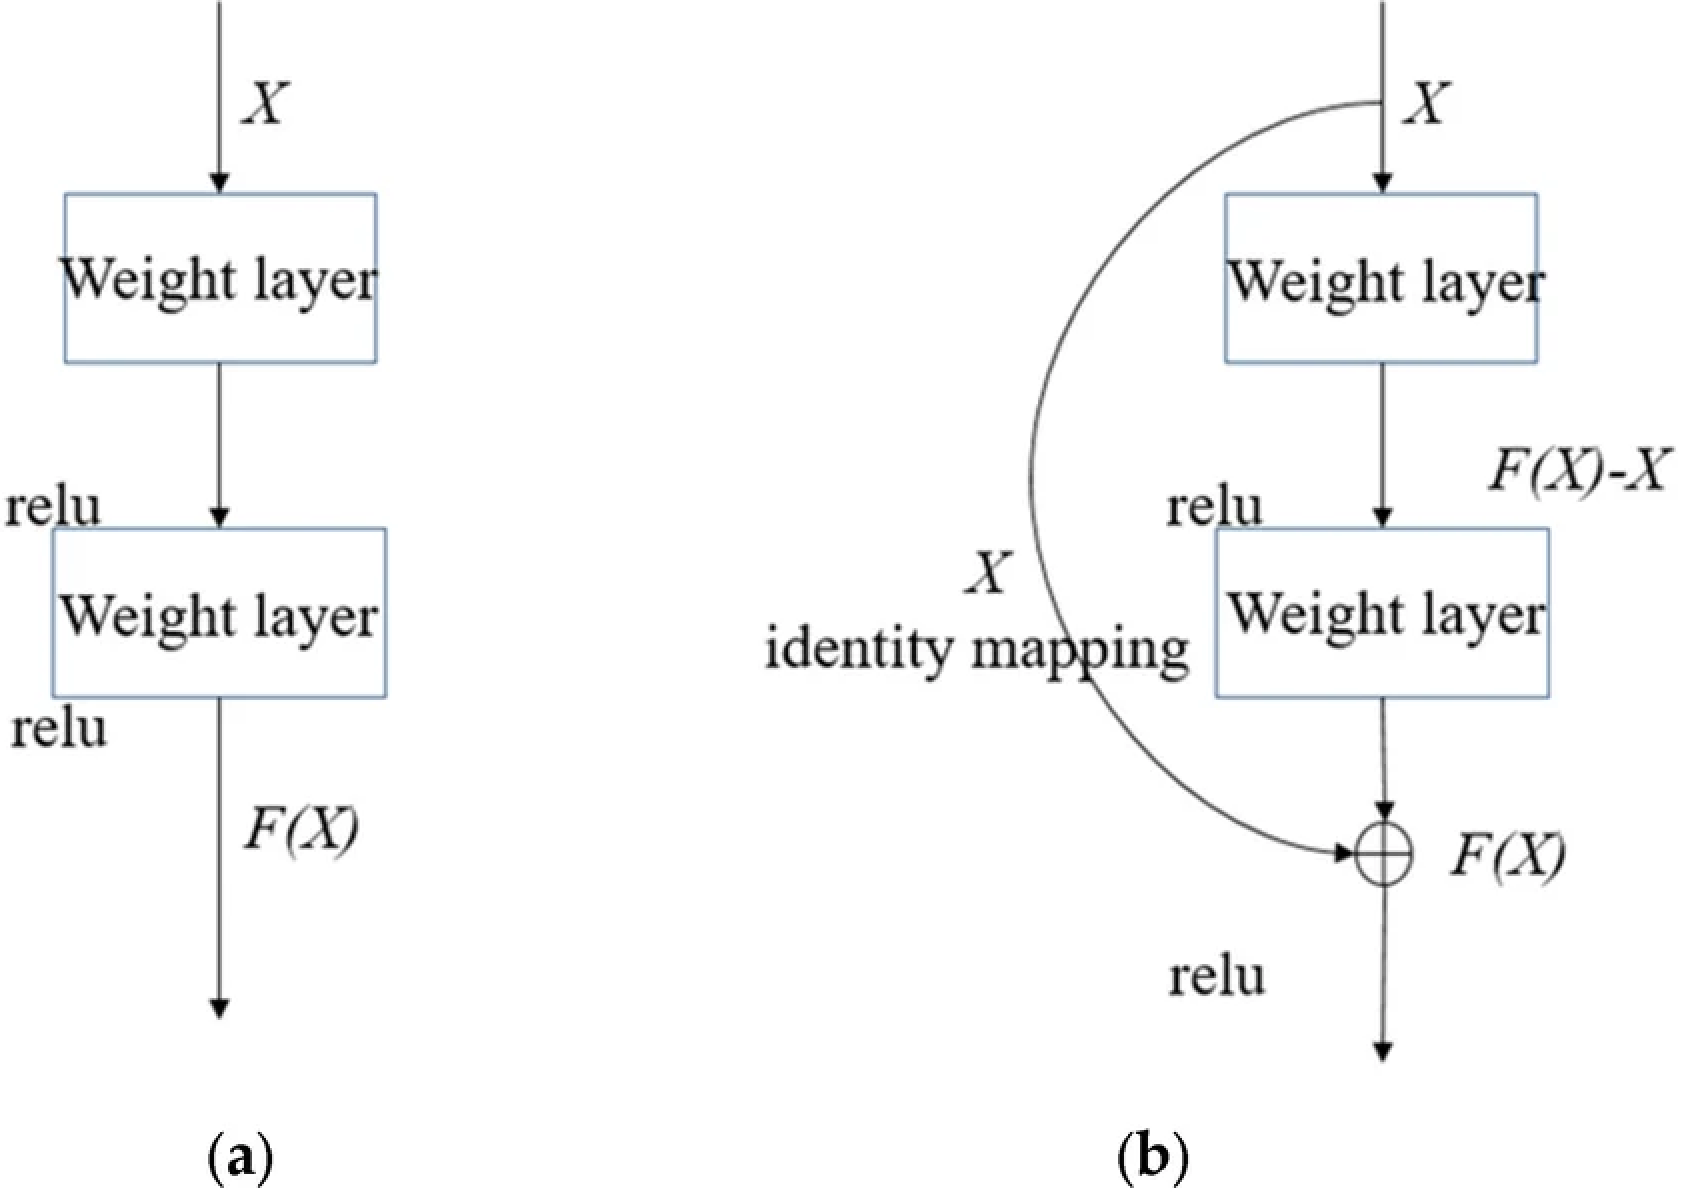
\includegraphics[width=\textwidth,height=2.08333in]{chapter0_img/resblock.png}

}

\subcaption{\label{fig-residual}Residual block and normal block}

\end{minipage}%
%
\begin{minipage}{0.50\linewidth}

\centering{

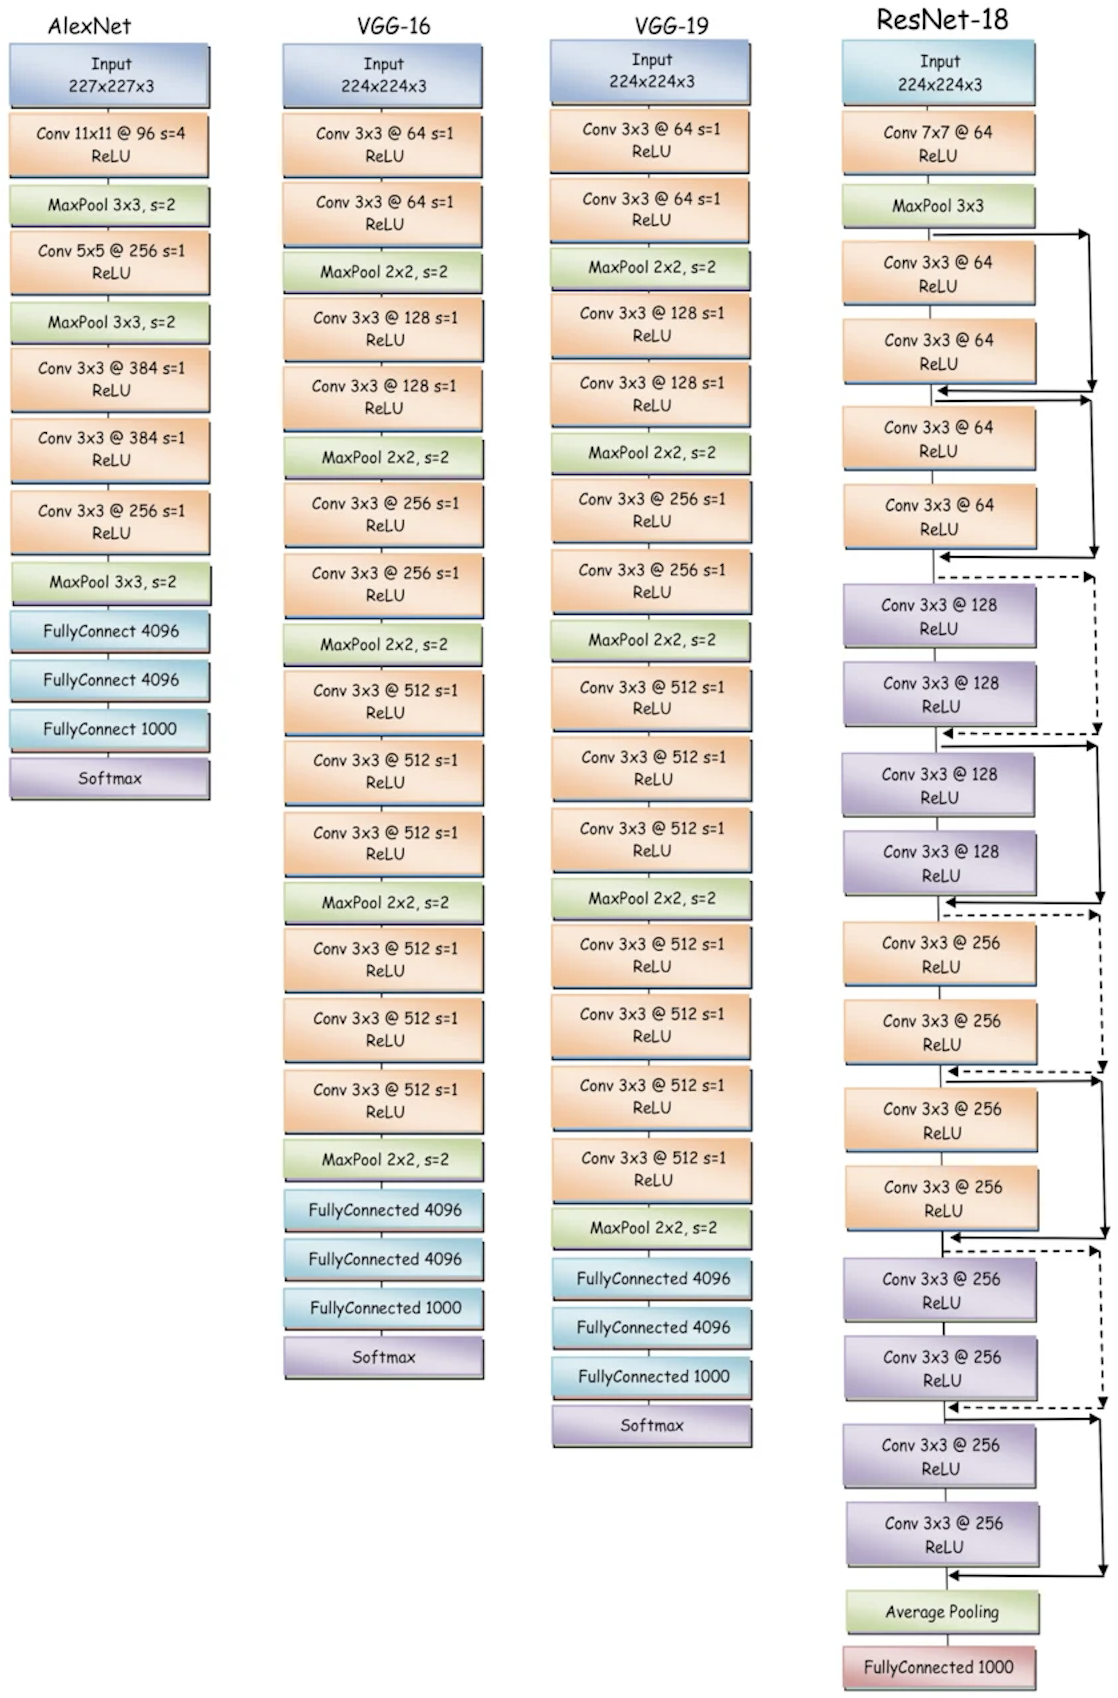
\includegraphics[width=\textwidth,height=2.08333in]{chapter0_img/layerdiff3.png}

}

\subcaption{\label{fig-difflayer3}Learnable depth: AlexNet (8 layers),
VGG-16 (16 layers), and ResNet-18 (18 layers)}

\end{minipage}%

\end{figure}%

\subsubsection{3.2.4 ViT}\label{vit}

While CNNs rely primarily on local convolutional operations to extract
visual features, the Vision Transforner
(ViT\textsuperscript{\citeproc{ref-vit}{6}}) introduced a different
approach that captures global dependencies across an image. Attention
weights are learned to represent relationships among image patches.
Unlike CNNs, which have inductive biases such as locality and
translation equivariance built into the architectures, ViT uses global
self-attention and imposes relatively little two-dimensional
neighborhood structure. Therefore, ViT performance can be more sensitive
to the amount of project-specific data。

These architectures were initially proposed as classification models,
which includes feature extraction and class prediction. The major
architectural difference lie in the feature extraction designs
(backbone) rather than the classification heads. The classification
heads serve a similar role to map extracted features to class
predictions.

Since backbone reflects the main architectual characteristics of models
designed for the same task, architecture names are commonly used to
describe the unique underlying feature extraction design when these
models are adapted as backbones for other tasks. For example, the same
detection framework can be implemented with different backbones, such as
VGG or ResNet, and these variants are often referred to by their
backbone architectures.

!!!!!!!!!!!!!!!!!!!!!!!!!!!! Representative backbones options for visual
feature learning, and it is therefore worthwhile to evaluate their
performance in classifying footwear characteristics.
!!!!!!!!!!!!!!!!!!!!!!!!

\section{4 CNN-based Object Detection}\label{cnn-based-object-detection}

To achieve the goal of the present study, footwear characteristics must
be both localized and classified to automate the process. Therefore, the
task is formulated as an object detection problem rather than an image
classification problem.

\subsection{4.1 Object Detection
Designs}\label{object-detection-designs}

In the detection workflow, the input image is first processed by a
visual backbone to extract feature representations. A detection head
then uses these representations to locate and classify target patterns.
Object detection models can be broadly categorized into two-stage and
one-stage models. Two-stage detectors first generate candidate regions
that may contain objects and then classify and refine these regions,
multiple networks are trained at the same time. Faster R-CNN is a
representative two-stage detector (Figure~\ref{fig-detections} upper
panel). In contrast, one-stage detectors predict object locations and
class labels directly from image features without a separate region
proposal stage (Figure~\ref{fig-detections} lower panel). YOLO models
are representative examples of this approach.

One-stage detectors simplified the architecture by excluding the
additional region proposal stage, this design reduces computational cost
and enables faster inference, making them suitable for real-time
applications. However, without a separate proposal and refinement
process, one-stage detectors may have relatively lower localization
accuracy compared with two-stage detectors. The present study does not
require real-time detection and prioritizes accurate localization,
Faster R-CNN was selected as the detector.

\begin{figure}

\centering{

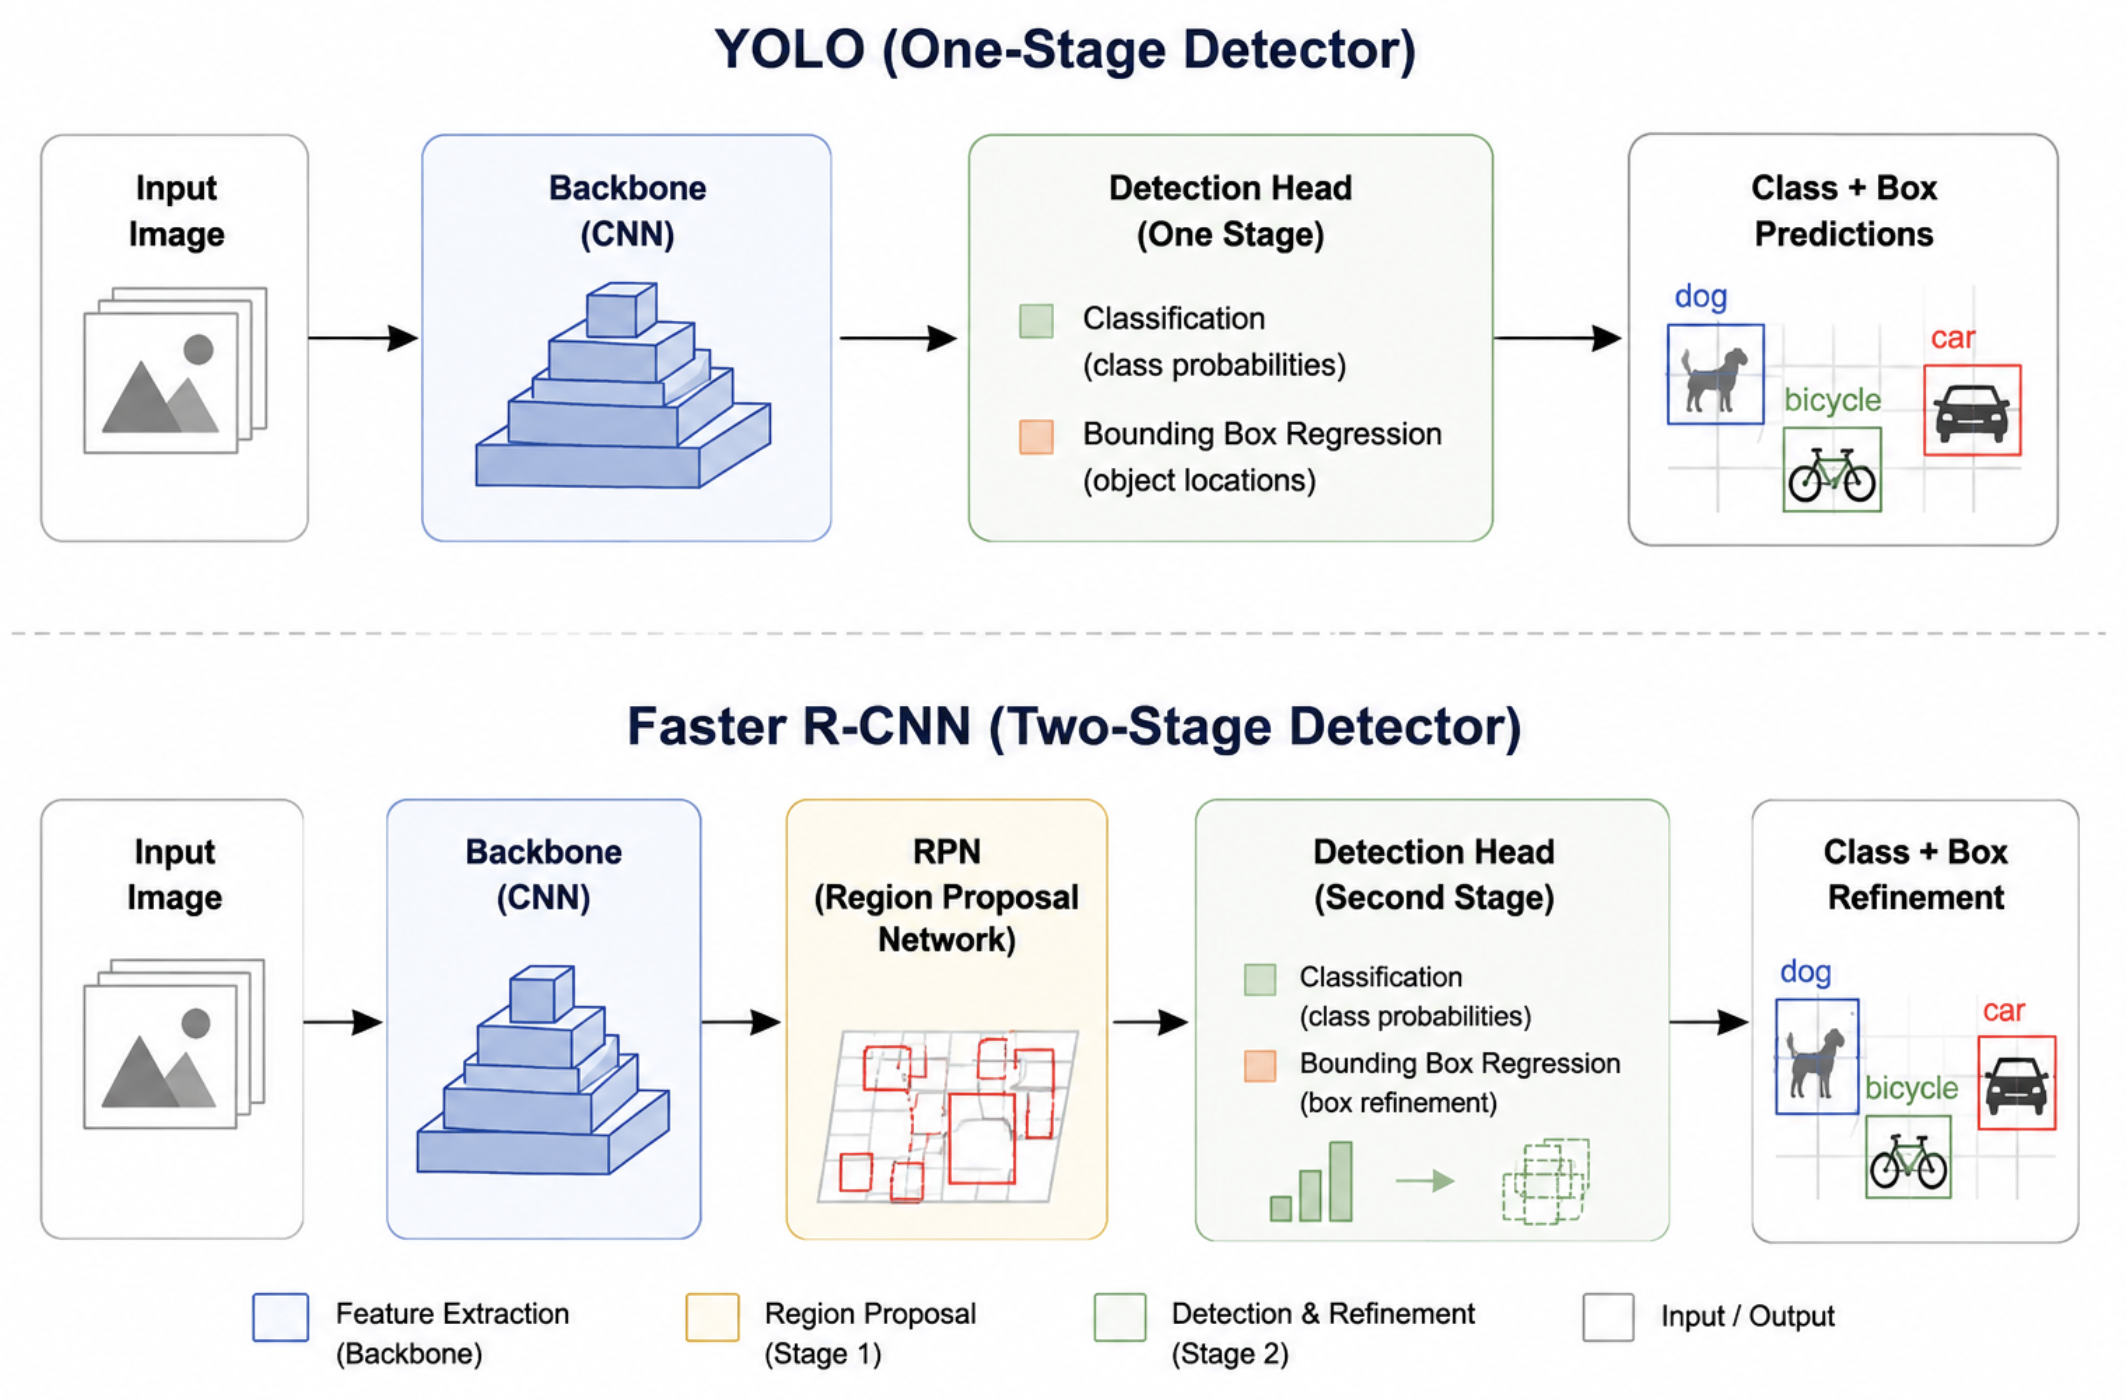
\includegraphics[width=\textwidth,height=2.08333in]{chapter0_img/detection2.png}

}

\caption{\label{fig-detections}One stage YOLO and two stage FasterRCNN}

\end{figure}%

\subsection{4.2 Faster R-CNN Backbones and
Heads}\label{faster-r-cnn-backbones-and-heads}

Faster R-CNN framework consisting of a backbone, a Region Proposal
Network (RPN), and a second-stage detection head. The backbone is
responsible for converting the input image into feature representations
that retain visual and spatial information in the image. Based on the
information, the RPN generates candidate regions that possibly contain
the objects. The candidate regions will be send into the detection head.
The detection head has two parallel branches: a classifier that predicts
categories for the regions, and a regressor that adjusts the coordinates
of the proposed box.

Faster R-CNN implementations can be realized by changing the backbone
while the overall framework remains unchanged. As mentioned previously,
backbone designs fundamentally affect the feature representations
provided to the detector, and consequently, detection performance.
Different backbone designs can provide different levels of semantic
abstraction and retained spatial
information\textsuperscript{\citeproc{ref-FPN}{14}}. The retained
spatial resolution is particularly important for localization because it
determines how much positional detail is preserved.

\subsection{4.3 Data}\label{data-1}

Object detection has a different data structure than the classification
task. To obtain the ability of predicting spatial location, the training
data must provide positional information in addition to the class label.
Input images are paired with these human-provided annotations, which
serve as the ground truth that guides model training and evaluation. For
example, in Figure~\ref{fig-2-detection-data}, the image is annotated
with both bounding boxes to indicate spatial locations as well as class
labels for objects in the bounding boxes. An individual object detection
image allows multiple target instances, each instance associates with a
class label and a spatial annotation. The annotated regions can belong
to the different classes, and it is common to find them overlap.

\begin{figure}

\centering{

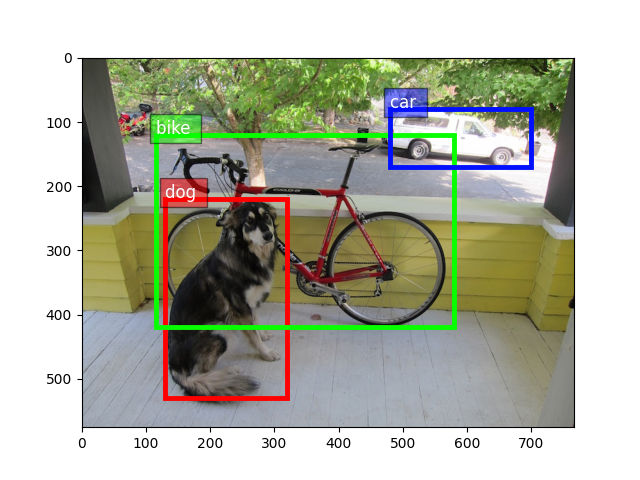
\includegraphics[width=3.01042in,height=\textheight]{chapter0_img/detection-data.png}

}

\caption{\label{fig-2-detection-data}Object detection data}

\end{figure}%

Low quality input would limit the network performance, hence, annotation
quality is an important consideration in object detection. Previous
studies have shown that small discrepancies in location annotation, such
as different box sizes, and noisy can influence localization
performance, especially for small
objects\textsuperscript{\citeproc{ref-annotatesize}{15}} because its
susceptibility to errors. In addition, deviation from intended
localization has been shown to reduce the detection performance of
Faster R-CNN\textsuperscript{\citeproc{ref-noisyannotation}{16}}.

\section{5 Relevance to the Present
Study}\label{relevance-to-the-present-study}

The footwear feature automation can be framed as an object detection
task that consists of two main stages: first locating footwear class
characteristics or patterns, and classifying the detected regions.
However, approaching the problem is more than adapting the network
architecture.

\subsection{5.1 Challenge}\label{challenge}

Object detection requires precisely annotated training data so that the
network can learn both spatial and categorical information. Previous
studies have reported that degraded annotation quality can significantly
reduce detection
performance\textsuperscript{\citeproc{ref-annotatesize}{15},\citeproc{ref-noisyannotation}{16}}.
Therefore, annotation quality is an important factor in network
performance.

Unlike general-purpose pretraining datasets, where object classes are
typically clearly defined, footwear features can be more complex and
ambiguous. For example, Figure~\ref{fig-brokencircle} shows a feature
coded as a ``circle'' in the forensic footwear tool SoleMate. However,
the feature itself consists of four individual arcs. It is therefore
open to discuss whether this feature should be annotated as one bounding
region labeled as a circle or as four separate regions labeled as arcs.

In addition to this ambiguity in grouping individual elements,
uncertainty can also arise from unclear boundaries between feature
categories. For example, Figure~\ref{fig-oval} and
Figure~\ref{fig-roundedbar} are coded as ``oval'' and ``bar with rounded
ends,'' respectively, and belong to two different categories. However,
the perceptual boundary between these categories may become unclear as
the shape is progressively elongated or compressed.

It is also difficult to exhaustively represent all possible feature
variants when the labeling system is restricted to a limited set of
basic categories such as circles, bars, and polygons. For example,
Figure~\ref{fig-knobbly} represents a variant of a circle. Numerous
visually different features may still be coded within the same
``circle'' category, making it impractical to collect examples of every
possible variant for model training.

\begin{figure}

\begin{minipage}{0.25\linewidth}

\centering{

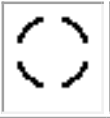
\includegraphics{chapter0_img/brokencircle.png}

}

\subcaption{\label{fig-brokencircle}A broken circle or four arcs}

\end{minipage}%
%
\begin{minipage}{0.25\linewidth}

\centering{


\includegraphics{chapter0_img/oval.png}

}

\subcaption{\label{fig-oval}Ellipse}

\end{minipage}%
%
\begin{minipage}{0.25\linewidth}

\centering{

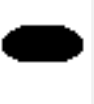
\includegraphics{chapter0_img/roundedbar.png}

}

\subcaption{\label{fig-roundedbar}A rounded bar}

\end{minipage}%
%
\begin{minipage}{0.25\linewidth}

\centering{

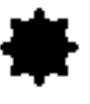
\includegraphics{chapter0_img/knobbly.png}

}

\subcaption{\label{fig-knobbly}A circle with a knobbly perimeter}

\end{minipage}%

\end{figure}%

\subsection{5.2 How Human Makes
Judgements}\label{how-human-makes-judgements}

A closer examination of the labeling process suggests that object
classes should be defined according to common human visual perception.
The trained network is intended to assist footwear examiners,
consistency between human interpretation and network labels is
important. For this reason, the classification labels should align with
human cognition in this study.

A ventral pathway is a pathway that process information that leads to
recognition and identification of objects. Visual information is
processed hierarchically along the ventral visual pathway. When human
sees an object, the eye-seeing signals first reach V1 area, where basic
features such as edges, orientations, and contrast are detected. These
signals then travel through the nervous system, they are reorganized in
a way so that they are received as an objects eventually. Gestalt
psychologists provide principles that explain how visual system
reorganize. According to Gestalt principle of
relatability\textsuperscript{\citeproc{ref-relatability}{17}} and
closure\textsuperscript{\citeproc{ref-gestalt}{18}}, the broken circle
(Figure~\ref{fig-brokencircle}) is perceived as a circle because the
curvatures are compatible, consequently the missing contour can be
interpolated and integrated into a continuous contour, and is perceived
as a circle. Even larger gap can be filled that a non-existing object is
perceived, the most famous example is the Kanizsa
trianglep\textsuperscript{\citeproc{ref-kanizsa}{19}}
(Figure~\ref{fig-Kanizsa}). In Figure~\ref{fig-Kanizsa}, although a
triangle whose edges are not physically present, human perceives the
boarder of a invisible triangle from the incomplete shapes.

\begin{figure}

\centering{

\includegraphics[width=3.01042in,height=\textheight]{chapter0_img/Kanizsatriangle.png}

}

\caption{\label{fig-Kanizsa}Kanizsa triangle}

\end{figure}%

Neuroscientific studies suggests that there are the connected neurons in
the primary cortex area (V1 area) compare their input, and they respond
to illusory edges in a similar way of responding to a real line.

In addition to the coherent perception, human also weighs global contour
organization and local features in the judgement. Loffler et
al.\textsuperscript{\citeproc{ref-loffler2003local}{20}} and Wilkinson
et al.\textsuperscript{\citeproc{ref-wilkinson1998detection}{21}}
studied smooth wave-like deformations of circles (radial frequency
change Figure~\ref{fig-RF1} Figure~\ref{fig-RF2}). They found observers
can detect very small shape changes, but when the contour is disrupted
or rearranged, performance drops strongly.
Wilson\textsuperscript{\citeproc{ref-wilson2015detection}{22}} studied
controlled deformations that gradually transform circles into polygons
(angular frequency change, Figure~\ref{fig-AF1} Figure~\ref{fig-AF2}),
they found jittering the contour has little effect, and performance on
single angle is close to performance on whole shape. Hence, curved
shapes rely more on global contour integration, whereas shapes with
corners rely more on local angle information. Weights of global and
local information are assigned differently for integration depending on
shape type when perceiving a shape.

\begin{figure}

\begin{minipage}{0.25\linewidth}

\centering{

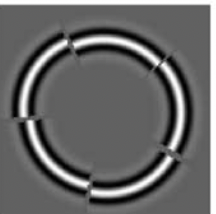
\includegraphics{chapter0_img/RF1.png}

}

\subcaption{\label{fig-RF1}circle jittering}

\end{minipage}%
%
\begin{minipage}{0.25\linewidth}

\centering{

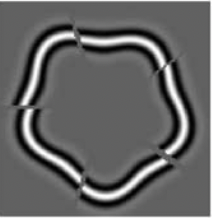
\includegraphics{chapter0_img/RF2.png}

}

\subcaption{\label{fig-RF2}RF5 jittering}

\end{minipage}%
%
\begin{minipage}{0.25\linewidth}

\centering{

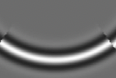
\includegraphics{chapter0_img/AF1.png}

}

\subcaption{\label{fig-AF1}circle segment}

\end{minipage}%
%
\begin{minipage}{0.25\linewidth}

\centering{


\includegraphics{chapter0_img/AF2.png}

}

\subcaption{\label{fig-AF2}AF5 segment}

\end{minipage}%

\caption{\label{fig-circle}~Radial and angular
deformations\textsuperscript{\citeproc{ref-wilkinson1998detection}{21}}
\textsuperscript{\citeproc{ref-wilson2015detection}{22}}\\
\emph{(a)-(b) jittering impairs discrimination suggesting RF (radial
frequency) perception depends n glnju9 obal contour arrangements}\\
\emph{(c)-(d) single angle has little effect on discrimination
suggesting AF (angular frequency) relies more on local features}}

\end{figure}%

\subsection{5.3 How the Problem Will be
Processed}\label{how-the-problem-will-be-processed}

Although visual networks have been developed for various purposes, their
ability to recognize footwear features has not been thoroughly
investigated. Footwear features present a particular challenge because
many of them can be represented as basic geometric elements, while human
perception of these elements is not always determined by strict
geometric definitions. This makes the task different from common
transfer-learning applications. CNNs incorporate several principles
inspired by biological visual processing, while attention-based models
focuses on attributing attention to more relevant features cross image
regions. Although this is not a direct model of human attention, the
adaptive weighting of relevant information is conceptually related to
selective attention in the human visual system. Therefore, we will
approach by examining whether visual networks can recognize geometric
footwear features in a manner consistent with human perception.
Specifically, we investigate their ability to extract basic geometric
elements, the effects of backbone depth and architectural
characteristics on feature representation, and whether networks trained
on predefined shape categories can recognize and classify shapes formed
through Gestalt perceptual organization.

\newpage

\section{6 Reference}\label{reference}

\phantomsection\label{refs}
\begin{CSLReferences}{0}{0}
\bibitem[\citeproctext]{ref-bodziak2017footwear}
\CSLLeftMargin{1. }%
\CSLRightInline{Bodziak, W. J. \emph{Footwear Impression Evidence:
Detection, Recovery and Examination}. (CRC Press, 2017).}

\bibitem[\citeproctext]{ref-Hubel1962}
\CSLLeftMargin{2. }%
\CSLRightInline{Awang, A. Receptive fields, binocular interaction and
functional architecture in the cat's visual cortex. \emph{The Journal of
physiology} (1962).}

\bibitem[\citeproctext]{ref-Hubel1965}
\CSLLeftMargin{3. }%
\CSLRightInline{Hubel, D. H. \& Wiesel, T. N. Receptive fields and
functional architecture in two nonstriate visual areas (18 and 19) of
the cat. \emph{Journal of neurophysiology} \textbf{28}, 229--289
(1965).}

\bibitem[\citeproctext]{ref-fukushima1980neocognitron}
\CSLLeftMargin{4. }%
\CSLRightInline{Fukushima, K. Neocognitron: A self-organizing neural
network model for a mechanism of pattern recognition unaffected by shift
in position. \emph{Biological cybernetics} \textbf{36}, 193--202
(1980).}

\bibitem[\citeproctext]{ref-transformer}
\CSLLeftMargin{5. }%
\CSLRightInline{Vaswani, A. \emph{et al.} Attention is all you need.
\emph{Advances in neural information processing systems} \textbf{30},
(2017).}

\bibitem[\citeproctext]{ref-vit}
\CSLLeftMargin{6. }%
\CSLRightInline{Dosovitskiy, A. \emph{et al.} An image is worth 16x16
words: Transformers for image recognition at scale. \emph{arXiv preprint
arXiv:2010.11929} (2020).}

\bibitem[\citeproctext]{ref-imagenet-transferlearning}
\CSLLeftMargin{7. }%
\CSLRightInline{Deng, J. \emph{et al.} Imagenet: A large-scale
hierarchical image database. in \emph{2009 IEEE conference on computer
vision and pattern recognition} 248--255 (Ieee, 2009).}

\bibitem[\citeproctext]{ref-transfer-learning}
\CSLLeftMargin{8. }%
\CSLRightInline{Yosinski, J., Clune, J., Bengio, Y. \& Lipson, H. How
transferable are features in deep neural networks? \emph{Advances in
neural information processing systems} \textbf{27}, (2014).}

\bibitem[\citeproctext]{ref-R-CNN}
\CSLLeftMargin{9. }%
\CSLRightInline{Girshick, R., Donahue, J., Darrell, T. \& Malik, J. Rich
feature hierarchies for accurate object detection and semantic
segmentation. in \emph{Proceedings of the IEEE conference on computer
vision and pattern recognition} 580--587 (2014).}

\bibitem[\citeproctext]{ref-vgg}
\CSLLeftMargin{10. }%
\CSLRightInline{Simonyan, K. \& Zisserman, A. Very deep convolutional
networks for large-scale image recognition. \emph{arXiv preprint
arXiv:1409.1556} (2014).}

\bibitem[\citeproctext]{ref-resnet}
\CSLLeftMargin{11. }%
\CSLRightInline{He, K., Zhang, X., Ren, S. \& Sun, J. Deep residual
learning for image recognition. in \emph{Proceedings of the IEEE
conference on computer vision and pattern recognition} 770--778 (2016).}

\bibitem[\citeproctext]{ref-alexnet}
\CSLLeftMargin{12. }%
\CSLRightInline{Krizhevsky, A., Sutskever, I. \& Hinton, G. E. Imagenet
classification with deep convolutional neural networks. \emph{Advances
in neural information processing systems} \textbf{25}, (2012).}

\bibitem[\citeproctext]{ref-layerdiff}
\CSLLeftMargin{13. }%
\CSLRightInline{He, K. \& Sun, J. Convolutional neural networks at
constrained time cost. in \emph{Proceedings of the IEEE conference on
computer vision and pattern recognition} 5353--5360 (2015).}

\bibitem[\citeproctext]{ref-FPN}
\CSLLeftMargin{14. }%
\CSLRightInline{Lin, T.-Y. \emph{et al.} Feature pyramid networks for
object detection. in \emph{2017 IEEE conference on computer vision and
pattern recognition (CVPR)} 936--944 (Ieee, 2017).}

\bibitem[\citeproctext]{ref-annotatesize}
\CSLLeftMargin{15. }%
\CSLRightInline{Murrugarra-Llerena, J., Kirsten, L. N. \& Jung, C. R.
Can we trust bounding box annotations for object detection? in
\emph{Proceedings of the IEEE/CVF conference on computer vision and
pattern recognition} 4813--4822 (2022).}

\bibitem[\citeproctext]{ref-noisyannotation}
\CSLLeftMargin{16. }%
\CSLRightInline{Wang, S., Gao, J., Li, B. \& Hu, W. Narrowing the gap:
Improved detector training with noisy location annotations. \emph{IEEE
Transactions on Image Processing} \textbf{31}, 6369--6380 (2022).}

\bibitem[\citeproctext]{ref-relatability}
\CSLLeftMargin{17. }%
\CSLRightInline{Kellman, P. J. \& Shipley, T. F. A theory of visual
interpolation in object perception. \emph{Cognitive psychology}
\textbf{23}, 141--221 (1991).}

\bibitem[\citeproctext]{ref-gestalt}
\CSLLeftMargin{18. }%
\CSLRightInline{Koffka, K. Principles of gestalt psychology. (1935).}

\bibitem[\citeproctext]{ref-kanizsa}
\CSLLeftMargin{19. }%
\CSLRightInline{Kanizsa, G. Subjective contours. \emph{Scientific
American} \textbf{234}, 48--53 (1976).}

\bibitem[\citeproctext]{ref-loffler2003local}
\CSLLeftMargin{20. }%
\CSLRightInline{Loffler, G., Wilson, H. R. \& Wilkinson, F. Local and
global contributions to shape discrimination. \emph{Vision research}
\textbf{43}, 519--530 (2003).}

\bibitem[\citeproctext]{ref-wilkinson1998detection}
\CSLLeftMargin{21. }%
\CSLRightInline{Wilkinson, F., Wilson, H. R. \& Habak, C. Detection and
recognition of radial frequency patterns. \emph{Vision research}
\textbf{38}, 3555--3568 (1998).}

\bibitem[\citeproctext]{ref-wilson2015detection}
\CSLLeftMargin{22. }%
\CSLRightInline{Wilson, H. R. \& Propp, R. Detection and recognition of
angular frequency patterns. \emph{Vision Research} \textbf{110}, 51--56
(2015).}

\end{CSLReferences}




\end{document}
